%!TEX root=../../main.tex

%\begin{doublespace}
\begin{spacing}{1.5}

\chapter{Foundations for inference}
\label{foundationsForInference}

On average, how many days a week are high school students physically active? How many hours of sleep per night do they get? These questions about the youth population in the United States could be answered either by collecting information from all 21.2 million high school aged youth (ages 15-19) or by formulating an estimate based on a well-chosen sample of students. The first strategy is simply impossible, while the second represents a primary goal of statistics -- drawing inferences about the characteristics of a population from a sample. In statistical terms, a characteristic of a population, such as the average amount of sleep per night for high school aged students, is called a \term{population parameter}. When carried out correctly, sampling from a population is an efficient way to estimate a population parameter. This chapter introduces the important ideas in drawing from samples by discussing methods of inference for a population mean, $\mu$ (Sections~\ref{variabilityInEstimates}-\ref{cltSection}). 

This chapter also discusses three widely used tools in statistics: point estimates (single number estimates) for a population mean, interval estimates that include a margin of error for point estimates, and a method for testing scientific hypotheses about $\mu$. The concepts used in this chapter will appear throughout later in the book. While particular equations or formulas may change to reflect the details of a problem at hand, the fundamental ideas will not. 

\index{data!yrbss|(}

One of the roles of the United States Centers for Disease Control and Prevention (CDC), as listed on their website, is "promoting healthy and safe behaviors, communities, and environment."\footnote{\url{http://www.cdc.gov/about/organization/mission.htm}} The first step in health promotion is to understand health behaviors; the CDC periodically conducts several surveys, including the Youth Risk Behavior Surveillance System (YRBSS).\footnote{\url{http://www.cdc.gov/healthyyouth/data/yrbs/index.htm}} Between 1991 and 2013, 2.6 million high school students have participated in more than 1,100 separate surveys. The next few sections discuss the \data{yrbss} dataset, which contains the responses of the 13,583 high school students who participated in the 2013 YRBSS.\footnote{\oiRedirect{textbook-yrbss}{www.cdc.gov/healthyyouth/data/yrbs/data.htm}} Part of this dataset is shown in Table~\ref{yrbssDF}, and the variables are described in Table~\ref{yrbssVariables}.

\begin{table}[h]
\centering
\begin{tabular}{rrllrrlrr}
  \hline
ID & age & gender & grade & height & weight & helmet & active & lifting \\ 
  \hline
1 &  14 & female & 9 &  &  & never &   4 &   0 \\ 
  2 &  14 & female & 9 &  &  & never &   2 &   0 \\ 
  3 &  15 & female & 9 & 1.73 & 84.37 & never &   7 &   0 \\ 
  $\vdots$ & $\vdots$ & $\vdots$ & $\vdots$ & $\vdots$ & $\vdots$ & $\vdots$ & $\vdots$ & $\vdots$ \\
  13582 &  17 & female & 12 & 1.60 & 77.11 & sometimes &   5 &  \\ 
  13583 &  17 & female & 12 & 1.57 & 52.16 & did not ride &   5 &  \\ 
  \hline
\end{tabular}
\caption{Five cases from the \data{yrbss} data set. Blank observations represent missing data. For example, the height and weight of students 1 and 2 are missing\textC{\vspace{-2mm}}}
\label{yrbssDF}
\end{table}
% library(openintro); library(xtable); data(yrbss); xtable(rbind(head(yrbss, 4), tail(yrbss, 2))[, c("age", "gender", "grade", "height", "weight", "helmet_12m", "physically_active_7d", "strength_training_7d")])

\begin{table}[h]
\centering\small
\begin{tabular}{l p{110mm}}
\hline
{\bf age} & {\bf Age of the student.} \\
\hline
\var{gender} & {Sex of the student.} \\
\var{grade} & Grade in high school (9-12) \\
\var{height} & Height, in meters. (1 m = ~3.28 ft) \\
\var{weight} & Weight, in kilograms (1 kg = ~2.2 lbs) \\
\var{helmet} & Frequency that the student wore a helmet while biking in the last 12~months. \\
\var{active} & Number of days physically active for 60+ minutes in the last 7 days. \\
\var{lifting} & Number of days of strength training (e.g. lifting weights) in the last 7 days. \\
\hline
\end{tabular}
\caption{Variables and their descriptions for the \data{yrbss} data set.}
\label{yrbssVariables}
\end{table}

\index{data!yrbss.samp|(}

CDC public health officials used the responses of 13,572 students to estimate the health behaviors of the \term{target population}: the approximately 21.2 million high school aged students in the US population. 

This chapter illustrates inference for a population mean by treating the CDC sample of 13,582 students as an artificial target population. A random sample of 100 participants (\data{yrbss.samp}) can then be used to estimate health behaviors for the "target population" of 13,572 respondents. In other words, this chapter will demonstrate how, with only the information from 100 students, it is possible to estimate the behaviors for 13,572 students (and by extension, show how the CDC used information from 13,572 students to estimate health behaviors for 21.2 million students).  

While the individuals in \data{yrbss} are not truly a target population, treating them as such allows for the estimates obtained by inference (using \data{yrbss.samp}) to be checked against the "population parameters" of \data{yrbss} -- not possible in a realistic setting, since population parameters (such as the average hours of sleep per night across 21.2 million students) are typically unknown.\footnote{Hence, the need for inference!}

The dataset \data{yrbss.samp} contains the data for 100 student responses randomly sampled from the larger \data{yrbss} dataset, and is described in Table~\ref{yrbssSampDF}.\footnote{About 10\% of high schoolers for each variable chose not to answer the question. Multiple regression (see Chapter~\ref{multipleAndLogisticRegression}) was used to predict what those responses would have been. For simplicity, we will assume that these predicted values are the unknown responses.} Histograms summarizing the \var{height}, \var{weight}, \var{active}, and \var{lifting} variables from \data{yrbss.samp} are shown in Figure~\ref{yrbssSampHistograms}.

\begin{table}
\centering
\begin{tabular}{rrllrrlrr}
  \hline
ID & age & gender & grade & height & weight & helmet & active & lifting \\ 
  \hline
5653 &  16 & female & 11 & 1.50 & 52.62 & never &   0 &   0 \\ 
  9437 &  17 & male & 11 & 1.78 & 74.84 & rarely &   7 &   5 \\ 
  2021 &  17 & male & 11 & 1.75 & 106.60 & never &   7 &   0 \\ 
  $\vdots$ & $\vdots$ & $\vdots$ & $\vdots$ & $\vdots$ & $\vdots$ & $\vdots$ & $\vdots$ & $\vdots$ \\
  2325 &  14 & male & 9 & 1.70 & 55.79 & never &   1 &   0 \\ 
   \hline
\end{tabular}
\caption{Four observations for the \data{yrbss.samp} data set, which represents a simple random sample of 100 high schoolers from the 2013 YRBSS.}
\label{yrbssSampDF}
% library(openintro); library(xtable); data(yrbss); xtable(rbind(head(yrbss.samp, 3), tail(yrbss.samp, 1))[, c("age", "gender", "grade", "height", "weight", "helmet_12m", "physically_active_7d", "strength_training_7d")])
%library(openintro); library(xtable); data(yrbss); data(yrbss.samp); xtable(yrbss.amp[c(1,2,3,100),])
\end{table}


% WARNING: This figure is referenced in Section 4.2
\begin{figure}
\centering
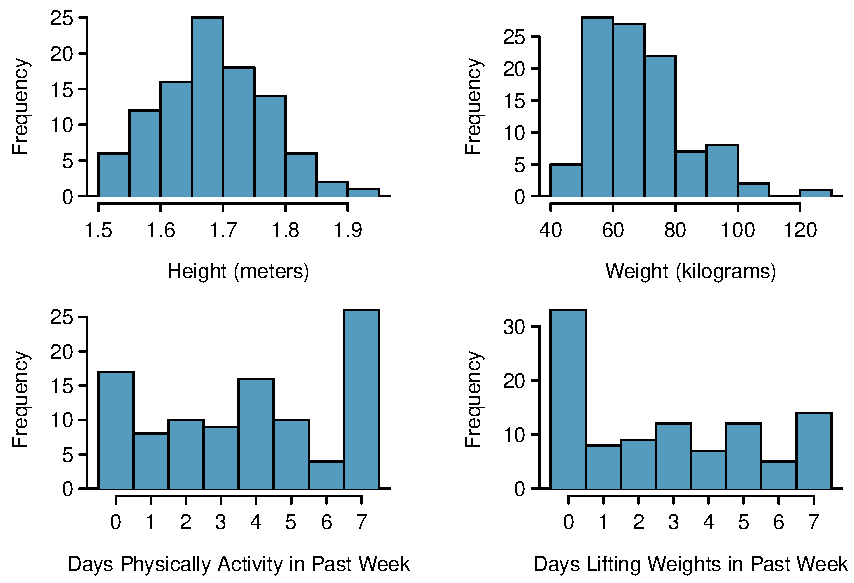
\includegraphics[width=0.8\textwidth]
{ch_inference_foundations_oi_biostat/figures/yrbssSampHistograms/yrbssSampHistograms} 
\caption{Histograms of \var{height}, \var{weight}, \var{activity}, and \var{lifting} for the sample data (\data{yrbss.samp}). The \var{height} distribution is approximately symmetric, \var{weight} is moderately skewed to the right, \var{activity} is bimodal or multimodal (with unclear skew), and \var{lifting} is strongly right skewed.\index{skew!example: moderate}\index{skew!example: strong}}
\label{yrbssSampHistograms}
\end{figure}

%__________________
\section[Variability in estimates]{Variability in estimates} %\sectionvideohref{youtube-DNIauUrRIEM&list=PLkIselvEzpM7Pjo94m1e7J5jkIZkbQAl4}}
\label{variabilityInEstimates}

\index{point estimate|(}

The \data{yrbss.samp} data can be used to estimate four features of the 13,582 high school students in \data{yrbss}: 1) average height, 2) average weight, 3) average number of days per week physically active (for more than 60 minutes at a time), 4) average body mass index (BMI).

Sample means are the natural choice of summary statistic for estimating a population mean. The average height of the students in \data{yrbss.samp} is:

\begin{align*}
\overline{x}_{height} = \frac{1.50 + 1.78 + \dots + 1.70}{100} = 1.697
\end{align*}
%library(openintro); data(yrbss.samp); mean(yrbss.samp$height); yrbss.samp$height

The sample mean $\overline{x} = 1.697$ meters (5 feet, 6.8 inches) is a \term{point estimate} of the population mean. If a second random sample of 100 were taken, the new sample mean would likely be different as a result of \term{sampling variation}.  Estimates generally vary from one sample to another, whereas the population mean is a fixed value; thus, the distinction between a sample mean versus a population mean is important. 

The sample means of \var{weight} and \var{active} provide estimates of the average weight and number of days active per week of YRBSS respondents. On average, students weigh 68.89 kilograms (about 151.6 pounds) and are active 3.75 days per week:
\begin{align*}
\overline{x}_{weight} &= \frac{52.6 + 74.8 + \dots + 55.8}{100} = 68.89
&\overline{x}_{active} &= \frac{0 + 7 + \dots + 1}{100} = 3.75.
\end{align*}
%library(openintro); data(yrbss.samp); d <- yrbss.samp$weight; mean(d); d
%library(openintro); data(yrbss.samp); d <- yrbss.samp$physically_active_7d; mean(d); d

BMI is used by health professionals to gauge whether an individual's weight is consistent with their height. While BMI is not one of the variables in the dataset, it can be calculated from height and weight (measured in metric units) with the formula:

\[bmi = \frac{weight}{height{^2}}\]

For example, the respondent with ID 5553 has BMI of 23.39 ($52.62/1.5^{2}$). Larger values of BMI indicate higher levels of body fat. Average BMI in \data{yrbss.samp} is found by calculating BMI values for each respondent, then computing the average of the BMI values. Average BMI in \data{yrbss.samp} is 23.92. Since adolescent size and body type can change with age, there are no population norms for BMI in the age range of YRBSS respondents as there are for adultss.

%%%  note that bmi cutpoints for children and teens are not the same as for adults. The CDC does not seem to recommend levels for health bmi for teens

Other population parameters, such as population median or population standard deviation, are also generally estimated using sample version. Table~\ref{ptEstimatesYrbssActive} shows estimates of the population mean, median, and standard deviation for respondents in \data{yrbss}, using \data{yrbss.samp}, as well as the "population parameters" calculated by using the full \data{yrbss} dataset. The estimates differ slightly from the population parameters, but not by much -- in fact, the estimate for median is equal to the population median. Note that the estimates will vary based on the sample taken; these estimates are specific to the data in \data{yrbss.samp}.

\begin{table}[h]
\centering
\begin{tabular}{ l rr}
\hline
\var{active}	& estimate & parameter  \\
\hline
mean		& 3.75 & 3.90 \\
median		& 4.00 & 4.00 \\
st. dev.		& 2.556 & 2.564 \\
\hline
\end{tabular}
\caption{Point estimates and parameter values for the \var{active} variable. The parameters were obtained by computing the mean, median, and SD for all respondents (i.e. the complete set of responses in \data{yrbss}).}
\label{ptEstimatesYrbssActive}
\end{table}

\begin{exercise} \label{peOfDiffActiveBetweenGender}
How would one estimate the difference in days active for men and women? If $\overline{x}_{men} = 4.3$ and $\overline{x}_{women} = 3.2$, then what is a good point estimate for the population difference?\footnote{If $\overline{x}_{men} = 4.3$ and $\overline{x}_{women} = 3.2$, the difference of the two sample means, $4.3 - 3.2 = 1.1$, would be an estimate of the difference. In other words, it can be concluded from the sample that on average, the male respondents are physically active about 1.1 days per week more than the female respondents.}
\end{exercise}
%library(openintro); library(xtable); data(yrbss); data(yrbss.samp); (x <- by(yrbss.samp$physically_active_7d, yrbss.samp$gender, mean)); diff(x)

While point estimates rarely equal population parameters (the median in Table~\ref{ptEstimatesYrbssActive} is one of those rare examples), they do become more accurate as more data become available. The running mean from the variable \var{active} in \data{yrbss.samp}, shown in Figure~\ref{yrbssActiveRunningMean}, demonstrates this principle. A \term{running mean} is a sequence of sample means in which each mean is calculated using one more observation than the mean preceding it in the sequence; in other words, sample size increases by 1 for each mean that is calculated. For example, the second mean in the sequence is the average of the first two observations, and the third mean in the sequence is the average of the first three observations. 

\begin{figure}[h]
   \centering
   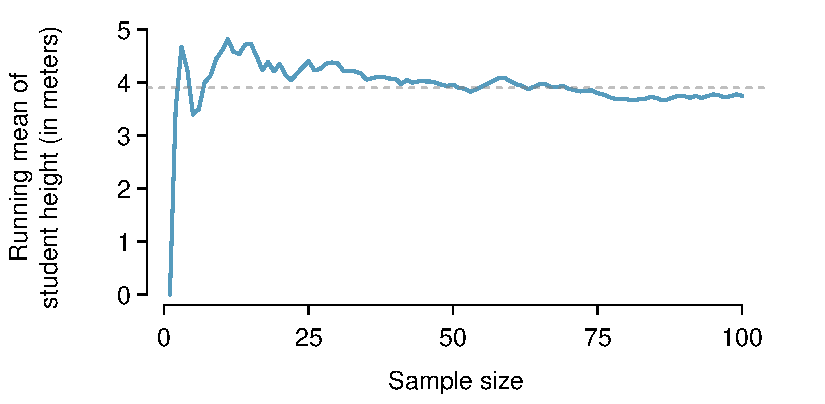
\includegraphics[width=0.72\textwidth]{ch_inference_foundations_oi_biostat/figures/yrbssActiveRunningMean/yrbssActiveRunningMean}
   \caption{The mean computed after gradually adding each individual to the sample (data from \data{yrbss.samp}). The mean tends to approach the true population average as more data become available. Running means calculated from a different random sample from \data{yrbss} would also show the same behavior.}
   \label{yrbssActiveRunningMean}
\end{figure}

\textit{DH: We should add the idea that AZ used in her draft: showing a different sequence of running means would show the same behavior.  Since we have only one sample here, not clear whether it is worth the added complexity.}

\textit{JV: I added that to the caption of the running mean figure. It may or may not be worth it to have a different random sample of 100 to prove the point -- both earlier, when pointing out that estimates are sample-specific, and then now, to illustrate how a different set of running means behaves the same way. If we did add it, it would be easy enough to partition Fig. 4.6 to show two graphs.}

As the sample size increases, the running mean approaches the true population mean of 3.90 days. Thus, the CDC officials can be reasonably confident that means calculated using data from 13,582 students can provide a good estimate of the true population mean across 21.2 million students. By using the formulas in the following section, Section~\ref{seOfTheMean}, it is possible to calculate how accurate sample estimates are likely to be.

\subsection{Standard error of the mean}
\label{seOfTheMean}

The point estimate $\overline{x} = 3.75$ days is an estimate of the population mean $\mu$ based on the random sample \data{yrbss.samp}. Another random sample of 100 participants might produce a different value of $\overline{x}$, such as 3.22 days; repeated random sampling would result in additional different values, perhaps 3.67 days, 4.10 days, and so on. Each sample mean can be thought of as a single observation from a random variable $\overline{X}$, that has the same kind of properties as discussed in Chapter 3. $\overline{X}$ will have a distribution of values, referred to as the \term{sampling distribution of the sample mean}; this distribution also has a mean and standard deviation.

In almost any study, such as those that produced the \data{LEAP} or \data{frog} datasets, conclusions about a population parameter must be drawn from the data collected, which represent a single sample. In those instances, the sampling distribution of $\overline{X}$ is a theoretical concept, not something that can be calculated -- obtaining repeated samples by conducting the studies again is simply not feasible or practical.

However, the concept can be illustrated here by taking repeated random samples from \data{yrbss}, the artificial population. Figure~\ref{yrbssActive1000SampDist} shows a histogram of sample means from 1,000 random samples of size 100 from \data{yrbss}. The histogram gives a picture of the theoretical sampling distribution of $\overline{X}$ when the sample size is 100. 

\begin{figure}[h]
   \centering
   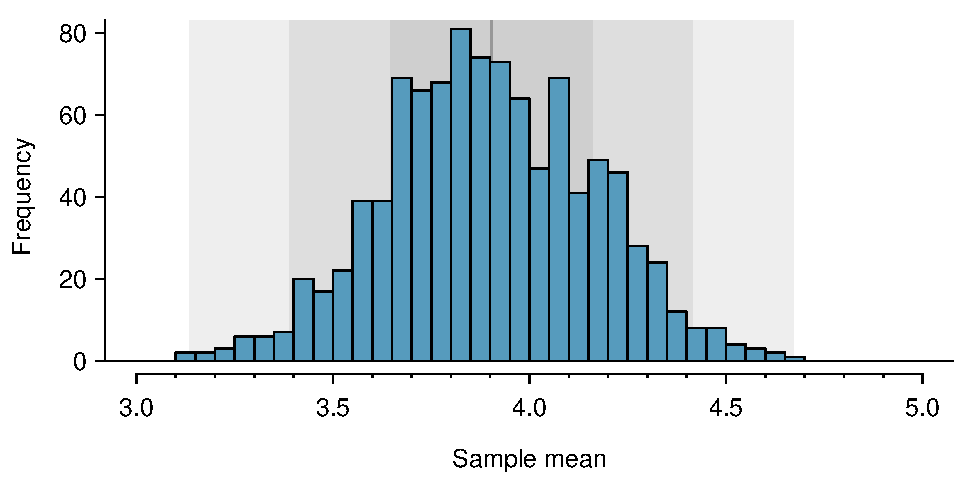
\includegraphics[width=0.9\textwidth]
{ch_inference_foundations_oi_biostat/figures/yrbssActive1000SampDist/yrbssActive1000SampDist}
   \caption{A histogram of 1000 sample means for number of days physically active per week, where the samples are of size $n=100$.}
   \label{yrbssActive1000SampDist}
\end{figure}

\begin{termBox}{\tBoxTitle{Sampling distribution}
The sampling distribution is the distribution of the point estimates based on samples of a fixed size from a certain population. It is useful to think of a particular point estimate as being drawn from such a distribution.}
\end{termBox}

The sampling distribution shown in Figure~\ref{yrbssActive1000SampDist} is unimodal and symmetric. The center of the histogram is approximately the mean of the random variable $\overline{X}$. Statistical theory can be used to show that the mean of the sampling distribution for $\overline{X}$ is exactly equal to the population mean. 

The \term{standard error} of the sample mean measures the sample-to-sample variability of $\overline{X}$, or in other words, the extent to which values of the repeated sample means oscillate around the population. The standard deviation of the 1,000 values of $\overline{X}$ is 0.26, approximately the standard error of $\overline{X}$. However, this method of estimating the standard error is not possible when there is only a single sample. Since the sample represents only one observation from $\overline{X}$, it cannot provide any information about the variability of the entire distribution.

The more realistic way to calculate standard error of the sample mean, when repeated random samples are not available, is to divide the population standard deviation ($\sigma_{x}$) by the square root of the sample size:

\[SE_{\overline{x}} = \sigma_{\overline{x}} = \dfrac{\sigma_{x}}{\sqrt{n}} = \dfrac{2.6}{\sqrt{100}} = 0.26\]

The probability tools of Section~\ref{randomVariablesSection} can be used to show that $\sigma_{\overline{X}} = \sigma/\sqrt{n}$. Conceptually, larger sample sizes result in sampling distributions that have decreasing variability; increasing $n$ for a given distribution with $\sigma_{x}$ will lower the standard error of the sample mean. In other words, increasing sample size causes $\overline{X}$ to be clustered more tightly around the population mean $\mu$, allowing for more accurate estimates of $\mu$ from a single sample.

% \term{standard error (SE)}\index{SE}\marginpar[\raggedright\vspace{-4mm}

% $SE$\\\footnotesize standard\\error]{\raggedright\vspace{-4mm}

% $SE$\\\footnotesize standard\\error} of the estimate.

\begin{termBox}{\tBoxTitle{The SE of the sample mean}
Given $n$ independent observations from a population with standard deviation $\sigma$, the standard error of the sample mean is equal to \vspace{-1mm}
\begin{align*}
SE = \frac{\sigma}{\sqrt{n}}
\label{seOfXBar}
\end{align*}\vspace{-3mm}%
}
\end{termBox}

However, the population standard deviation $\sigma$ is typically unknown. Instead, the sample standard deviation $s$ can be used as a reasonably good estimate of $\sigma$, and $s / \sqrt{n}$ as an estimate for the standard error of the sample mean. For example, the estimate of SE using \data{yrbss.samp} is 0.2556 ($2.556 / \sqrt{100}$), which is very close to 0.26.

This estimate tends to be sufficiently good when the sample size is at least 30 and the population distribution is not strongly skewed. In the case of skewed distributions, a larger sample size is necessary. These topics are further discussed in Section~\ref{cltSection}.

%\begin{comment}
The terminology for point estimates can be confusing, and is worth restating:  

\begin{itemize}
	
	\item The population parameters $\mu$ and $\sigma$ are characteristics of the target population from which a sample is drawn. 
	
	\item In a single sample, the arithmetic average of the values in the sample (the sample mean) is denoted by $\overline{x}$. The sample standard deviation is denoted by $s$. 
	
	\item If repeated samples could be taken, the random variable $\overline{X}$ represents the collection of sample means (one for each sample). The distribution of $\overline{X}$ is called its sampling distribution, which itself has a mean and standard deviation. 
	
	\item With random sampling, the mean of the random variable $\overline{X}$ is always equal to the population mean $\mu$.  In the notation of Chapter 3, $\mu_{\overline{X}} = E(\overline{X}) = \mu$.
	
	\item  The standard deviation of $\overline{X}$, written $\sigma_{\overline{X}}$, is called its standard error (SE). 
	
	\item The standard error of the sample mean, as calculated from a single sample of size $n$, is equal to $\dfrac{\sigma}{\sqrt{n}}$. SE can be estimated by using $s$, such that $SE = \dfrac{s}{\sqrt{n}}$.
	
\end{itemize}

%\end{comment}

\index{point estimate|)}

\section[Confidence intervals]{Confidence intervals} %\sectionvideohref{youtube-FUaXoKdCre4&list=PLkIselvEzpM7Pjo94m1e7J5jkIZkbQAl4}}
\label{confidenceIntervals}
\subsection{Interval estimates for a population parameter}

A \term{confidence interval} provides an estimate for a population parameter along with a margin of error, giving a plausible range of values for the parameter instead of a single value. When estimating a population mean $\mu$, a confidence interval for $\mu$ has the general form

\[(\overline{x} -m, \ \overline{x} + m) = \overline{x} \pm m \],
where $m$ is the margin of error. The standard error, a measure of the uncertainty associated with the point estimate, is used in the calculation of the margin of error.

\subsection{An approximate 95\% confidence interval}

The standard error of the sample mean is its standard deviation; thus, by the empirical rule discussed in Section~(\ref{}) of Chapter 3, the sample mean will be within 2 standard errors of the population mean $\mu$ approximately 95\% of the time. If an interval is constructed that spans 2 standard errors from the point estimate in either direction, a data analyst can be 95\% \term{confident} that the population mean is somewhere within the interval:

\begin{align}
\text{point estimate}\ \pm\ 2\times SE
\label{95PercentConfidenceIntervalFormula}
\end{align}

The phrase "95\% confident" has a subtle interpretation: if many samples were drawn from a population, with each one used to calculate a confidence interval using Equation~\ref{95PercentConfidenceIntervalFormula}, about 95\% of those intervals would contain the population mean $\mu$. Figure~\ref{95PercentConfidenceInterval} illustrates this process with 25 samples taken from \data{yrbss}. 24 of the resulting confidence intervals contain the average number of days per week that respondents are physically active, $\mu$ = 3.90 days, while one interval does not. 

Just as with the sampling distribution of the sample mean, the interpretation of a confidence interval relies on the abstract construct of repeated sampling. A data analyst, who can only observe one sample, does not know whether the population mean lies within the single interval calculated. However, the concept behind the calculation implies that approximately 95 intervals out of 100 will contain the population mean. The value 95\% is an approximation, accurate when the sampling distribution for the sample mean is close to that of a normal distribution. This assumption holds when the sample size is sufficiently large, as will be shown later.

\begin{figure}[hht]
   \centering
   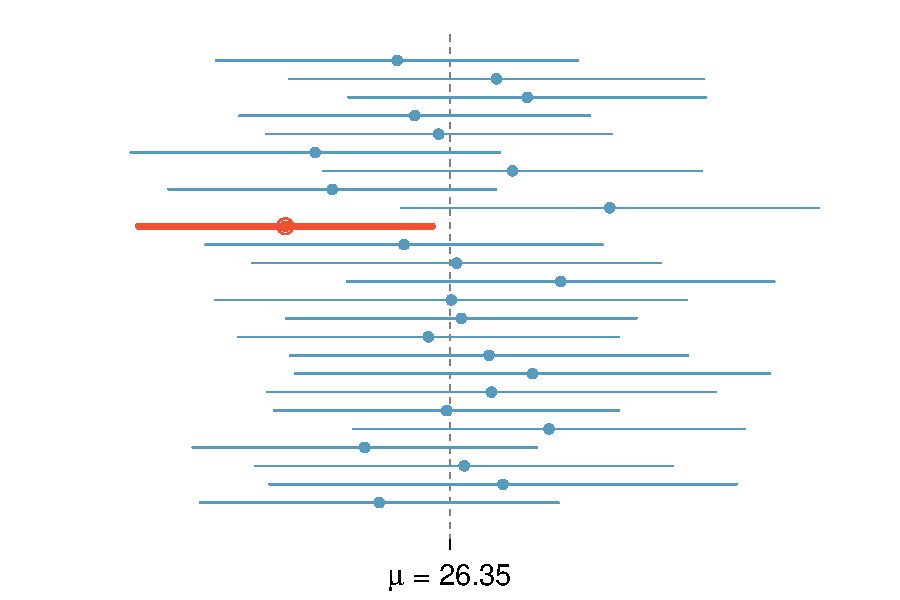
\includegraphics[width=0.78\textwidth]
{ch_inference_foundations_oi_biostat/figures/95PercentConfidenceInterval/95PercentConfidenceInterval}
   \caption{Twenty-five samples of size $n=100$ were taken from \data{yrbss}. For~each sample, a confidence interval was created to try to capture the average number of days per week that students are physically active. Only~1 of these~25 intervals did not capture the true mean, $\mu = 3.90$~days.}
   \label{95PercentConfidenceInterval}
\end{figure}

\begin{exercise}
In Figure~\ref{95PercentConfidenceInterval}, one interval does not contain 3.90 minutes. Does this imply that the mean cannot be 3.90?\footnote{Just as some observations occur more than 2 standard deviations from the mean, some point estimates will be more than 2 standard errors from the parameter. A confidence interval only provides a plausible range of values for a parameter. While we might say other values are implausible based on the data, this does not mean they are impossible.}
\end{exercise}

\begin{example}{The sample mean of days active per week from \data{yrbss.samp} is 3.75~days. The standard error, as estimated using the sample standard deviation, is $SE=\frac{2.564}{\sqrt{100}} = 0.2564$~days. Calculate a 95\% confidence interval for the average days active per week for all YRBSS students.}
We apply Equation~\ref{95PercentConfidenceIntervalFormula}:
\[3.75\ \pm\ 2 \times  0.26 \quad \rightarrow \quad (3.23, 4.27)\]
Based on these data, we can be about 95\% confident that the average days active per week for all YRBSS students was larger than 3.23 but less than 4.27~days. The interval extends out 2 standard errors from the point estimate, $\overline{x}_{active}$.
\end{example}
% library(openintro); library(xtable); d <- yrbss.samp; mean(d$physically_active_7d); sd(d$physically_active_7d); sd(yrbss$physically_active_7d, na.rm=TRUE)

\begin{exercise} \label{95CIExerciseForAgeOfYrbssSamp1}
The sample data suggest that the average YRBSS student height is $\overline{x}_{height} = 1.697$ meters with a standard error of 0.0088 meters (estimated using the sample standard deviation, 0.088 meters). What is an approximate 95\% confidence interval for the average height of all of the YRBSS students?\footnote{Apply Equation~\ref{95PercentConfidenceIntervalFormula}: $1.697 \ \pm \ 2\times 0.0088 \rightarrow (1.6794, 1.7146)$.  We are about 95\% confident the average height of all YRBSS students was between 1.6794 and 1.7146 meters (5.51~to 5.62~feet).}
\end{exercise}
% library(openintro); d <- yrbss.samp; mean(d$height); sd(d$height)

\subsection{The sampling distribution for the mean}

Section~\ref{seOfTheMean} introduced the notion of the sampling distribution for $\overline{X}$, the average number of days physically active per week for samples of size 100. Figure~\ref{yrbssActive1000SampDist} showed the distribution of sample means calculated from 1,000 random samples. Since the complete sampling distribution consists of means for all possible samples of size 100, drawing a much larger number of samples would provide a more accurate view of the distribution; the left panel of Figure~\ref{yrbssActiveBigSampDist} shows the distribution calculated from 100,000 sample means. 

\begin{figure}[hht]
   \centering
   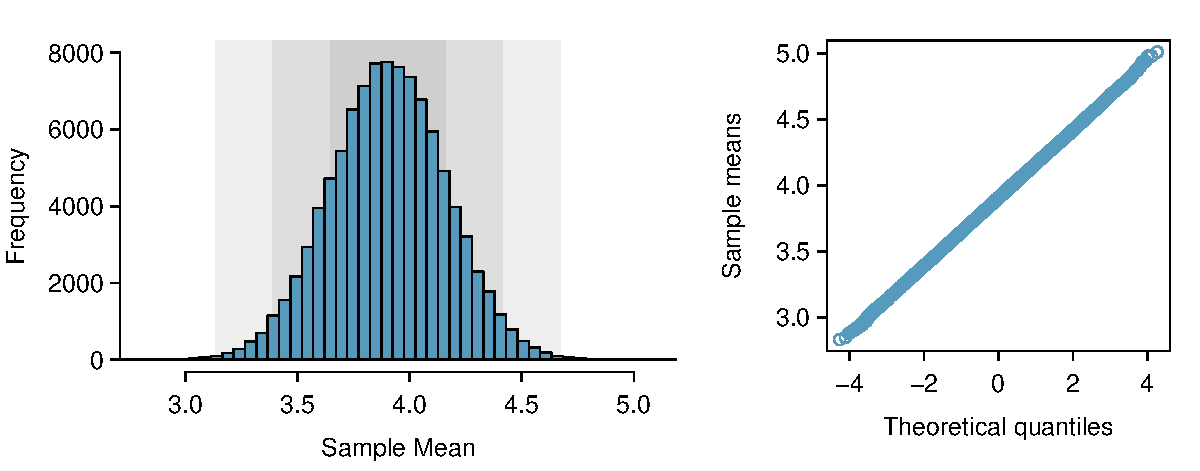
\includegraphics[width=\textwidth]
{ch_inference_foundations_oi_biostat/figures/yrbssActiveBigSampDist/yrbssActiveBigSampDist}
   \caption{The left panel shows a histogram of the sample means for 100,000 random samples. The right panel shows a normal probability plot of those sample means.}
   \label{yrbssActiveBigSampDist}
\end{figure}

%\textit{Normal probability plots are covered in Chap 3}

The distribution of sample means closely resembles the normal distribution (see Section~\ref{normalDist}). A normal probability plot of these sample means is shown in the right panel of Figure~\ref{yrbssActiveBigSampDist}. All of the points closely fall around a straight line, implying that  the distribution of sample means is nearly normal. This result can be explained by the Central Limit Theorem.

\begin{termBox}{\tBoxTitle{Central Limit Theorem, informal description}
If a sample consists of at least 30 independent observations and the data are not strongly skewed, then the distribution of the sample mean is well approximated by a~normal model.\index{Central Limit Theorem}}
\end{termBox}

% We will apply this informal version of the Central Limit Theorem for now, and discuss its details further in Section~\ref{cltSection}.

The choice 2 standard errors in Equation~(\ref{95PercentConfidenceIntervalFormula}) was based on the general guideline that roughly 95\% of the time, observations are within two standard deviations of the mean. Under the normal model, this can be made more accurate by using 1.96 in place~of~2.
\begin{eqnarray}
\text{point estimate}\ \pm\ 1.96\times SE
\label{95PercentCIWhenUsingNormalModel}
\end{eqnarray}
% If a point estimate, such as $\overline{x}$, is associated with a normal model and standard error $SE$, then we use this more precise 95\% confidence interval.

%%%% revisions to  here, 24 nov 2015

\subsection{Changing the confidence level}
\label{changingTheConfidenceLevelSection}

\index{confidence interval!confidence level|(}

Ninety-five percent confidence intervals are the most commonly used interval estimates, but confidence intervals with confidence levels different from 95\% are straightforward to construct.  A general 95\% confidence interval for a point estimate that comes from a nearly normal distribution is 
\begin{eqnarray}
\text{point estimate}\ \pm\ 1.96\times SE
\end{eqnarray}
There are three components to this interval: the point estimate; ``1.96''; and the standard error. The choice of $1.96\times SE$ was based on capturing 95\% of the distribution of the sample mean,  since the estimate is within 1.96 standard deviations of the parameter about 95\% of the time. 

\begin{exercise} \label{leadInForMakingA99PercentCIExercise}
If $Y$ is a normally distributed random variable, how often will $Y$ be within 2.58 standard deviations of the mean?\footnote{This is equivalent to asking how often the Z-score will be larger than -2.58 but less than 2.58. (For a picture, see Figure~\ref{choosingZForCI}.) To determine this probability, look up -2.58 and 2.58 in the normal probability table (0.0049 and 0.9951). Thus, there is a $0.9951-0.0049 \approx 0.99$ probability that the unobserved random variable $Y$ will be within 2.58 standard deviations of $\mu$.}
\end{exercise}

To create a 99\% confidence interval, change 1.96 in the 95\% confidence interval formula to  $2.58$. Guided Practice~\ref{leadInForMakingA99PercentCIExercise} highlights that 99\% of the time a normal random variable will be within 2.58 standard deviations of the mean. This approach -- using the $Z$-scores in the normal model to compute confidence levels -- is appropriate when $\overline{x}$ is associated with a normal distribution with mean $\mu$ and standard deviation $SE_{\overline{x}}$. Thus, the formula for a 99\% confidence interval is
\begin{eqnarray}
\overline{x}\ \pm\ 2.58\times SE_{\overline{x}}
\label{99PercCIForMean}
\end{eqnarray}

A data analyst can be 99\% confident that this wider interval contains the population mean.


\begin{figure}[h]
\centering
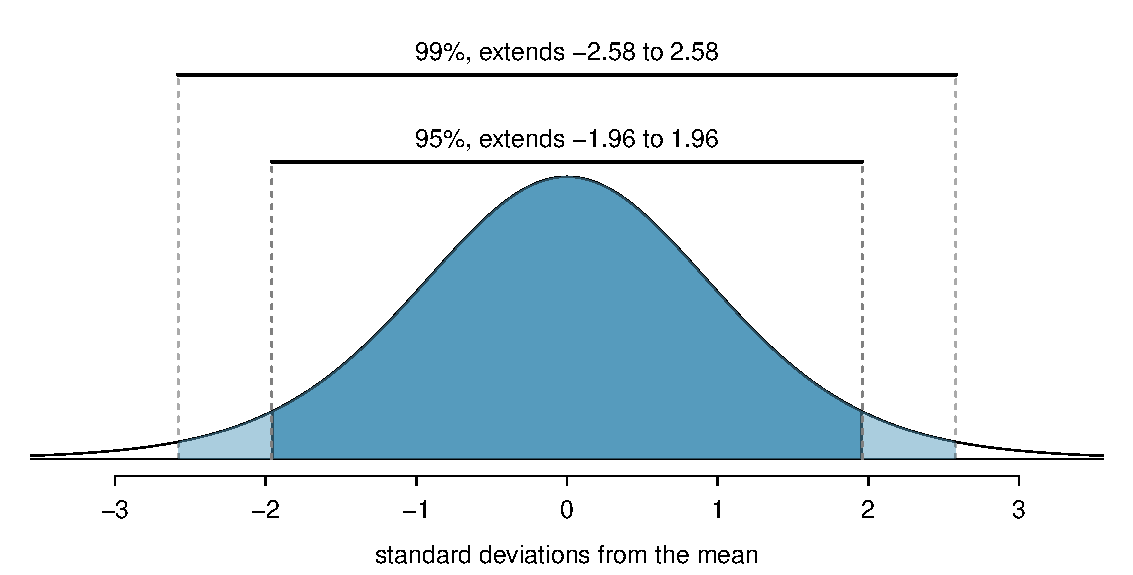
\includegraphics[width=\textwidth]
{ch_inference_foundations_oi_biostat/figures/choosingZForCI/choosingZForCI}
\caption{The area between -$z^{\star}$ and $z^{\star}$ increases as $|z^{\star}|$ becomes larger. If the confidence level is 99\%, $z^{\star}$ is chosen such that 99\% of the normal curve is between -$z^{\star}$ and $z^{\star}$, which corresponds to 0.5\% in the lower tail and 0.5\% in the upper tail: $z^{\star}=2.58$.}
\label{choosingZForCI}
\index{confidence interval!confidence level|)}
\end{figure}

The normal approximation is crucial to the precision of these confidence intervals. Section~\ref{cltSection} provides a more detailed discussion about when the normal model can safely be applied. When the normal model is not a good fit,  alternative distributions that better characterize the sampling distribution will be used.

\textit{when do these alternative distributions appear?}

\begin{termBox}{\tBoxTitle{Conditions for $\overline{X}$ being nearly normal and $SE$ being accurate\label{terBoxOfCondForXBarBeingNearlyNormalAndSEBeingAccurate}}
Important conditions to help ensure the sampling distribution of $\overline{X}$ is nearly normal and the estimate of SE sufficiently accurate:
\begin{itemize}
\setlength{\itemsep}{0mm}
\item The sample observations are independent.
\item The sample size is large: $n\geq30$ is a good rule of thumb.
\item The population distribution is not strongly skewed. 
\end{itemize}
For sample sizes larger than about 45, the condition on skewness can be ignored, unless there are prominent outliers in the sample. }
\end{termBox}

\begin{tipBox}{\tipBoxTitle[]{How to verify sample observations are independent}
If the observations are from a simple random sample and consist of fewer than 10\% of the population, then they are independent.\\[2mm]
Subjects in an experiment are considered independent if they undergo random assignment to the treatment groups. \\[2mm]
}
\end{tipBox}

\begin{tipBox}{\tipBoxTitle[]{Checking for strong skew usually means checking for obvious outliers}
When there are prominent outliers present, the sample should contain at least 100 observations, and in some cases, much more. \\[2mm]
}
\end{tipBox}

% WARNING !!!!
% EOCE 4.9 (as of 2nd Edition) references the results of this exercise
\begin{exercise} \label{find99CIForYrbssAgeExercise}
Create a 99\% confidence interval for the average days active per week of all YRBSS students using \data{yrbss.samp}. The point estimate is $\overline{x}_{active} = 3.75$ and the standard error is $SE_{\overline{x}} = 0.26$.\footnote{The observations are independent (simple random sample, $<10\%$ of the population), the sample size is at least 30 ($n = 100$), and the distribution doesn't have a clear skew (Figure~\ref{yrbssSampHistograms} on page~\pageref{yrbssSampHistograms}); the normal approximation and estimate of SE should be reasonable. Apply the 99\% confidence interval formula: $\overline{x}_{active}\ \pm\ 2.58 \times  SE_{\overline{x}} \rightarrow (3.08, 4.42)$. We are 99\% confident that the average days active per week of all YRBSS students is between 3.08 and 4.42~days.}
\end{exercise}
%library(openintro); data(yrbss.samp); d <- yrbss.samp; mean(d$age); sd(d$age)/sqrt(100)

\begin{termBox}{\tBoxTitle{Confidence interval for any confidence level}
If the point estimate follows the normal model with standard error $SE$, then a confidence interval for the population parameter is
\begin{eqnarray*}
\text{point estimate}\ \pm\ z^{\star} SE
\end{eqnarray*}
where $z^{\star}$ corresponds to the confidence level selected.}
\end{termBox}

Figure~\ref{choosingZForCI} provides a picture of how to identify $z^{\star}$ based on a confidence level. We~select $z^{\star}$ so that the area between -$z^{\star}$ and $z^{\star}$ in the normal model corresponds to the confidence level. 

\begin{termBox}{\tBoxTitle{Margin of error}
\label{marginOfErrorTermBox}In a confidence interval, $z^{\star}\times SE$ is called the \term{margin of error}.}
\end{termBox}

\textC{\newpage}

\begin{exercise} \label{find90CIForYrbssAgeExercise}
Use the data in Guided Practice~\ref{find99CIForYrbssAgeExercise} to create a 90\% confidence interval for the average days active per week of all YRBSS students.\footnote{First find $z^{\star}$ such that 90\% of the distribution falls between -$z^{\star}$ and $z^{\star}$ in the standard normal model, $N(\mu=0, \sigma=1)$. The value -$z^{\star}$ is found in the normal probability table by looking for a lower tail of 5\% (the other 5\% is in the upper tail): $z^{\star}=1.65$. The 90\% confidence interval is $\overline{x}_{active}\ \pm\ 1.65\times SE_{\overline{x}} \to (3.32, 4.18)$. (The conditions for  conditions for normality and the standard error were verified in the earlier example.)  
We are 90\% confident the average days active per week is between 3.32 and 4.18~days.}

\end{exercise}


\subsection{Interpreting confidence intervals}
\label{interpretingCIs}

\index{confidence interval!interpretation|(}

National Health and Nutrition Examination Survey (NHANES) consists of a set of surveys and measurements conducted by the US CDC to assess the health and nutritional status of adults and children in the United States. NHANES is unique in that it combines interviews and physical examinations.  The dataset \data{nhanes.samp} contains 76 variables and is a random sample 200 individuals from the measurements in 2009-2010 and 2012-2013 sample years.  The sample was drawn from a large sample of 20,293 participants available in the package \textbf{NHANES} available from The Comprehensive R Archive Network~\footnote{http://cran.us.r-project.org} (CRAN).  The CDC uses a complex sampling design that samples some demographic subgroups with larger probabilities, but \data{nhanes.samp} has been adjusted so that it can be viewed as a random sample of the US population.  

As noted earlier, there are no population norms for bmi for adolescents, but by adulthood, an  individual's height and weight should be stable, so body mass index for people age 21 and older is often used as a measure body fat that can be compared to population norms or between gender. Both age and body mass index (bmi) are available on the dataset and can be used to estimate mean bmi in the US population for the years represented by \data{nhanes.samp}

\textit{should we list sample variables as in ch 1, or just plunge in?  I think we should just plunge in.  We should make the data available, though}

\begin{example}{Use \data{nhanes.samp} to calculate a 95\% confidence interval for adult bmi in the US population. \label{exNhanesBmi}}
	In the random sample of 200 participants, 152 are age 21 years or older and bmi is available for 151 of these 152 participants.  The distribution of bmi is shown in the histogram for the variable \var{BMI} shown in Figure~\ref{nhanesAdultBmiHist}.  The histogram shows some right-skewness in the data, and one large outlier.  The outlier has value 81.3 and corresponds to an individual with weight 230.7kg (508.6 lbs) and height 168.5cm (66.3in). In an initial analysis of a dataset like this one, a value of bmi this large would be checked for accuracy. It could correspond to an unexpectedly large adult or an error in recording data.  Since accuracy cannot be checked in the data available on CRAN, the analysis here assumes that that weight there is an error in the weight recorded for this individual and the data point has been dropped, producing a sample size of 150. 
	
	The mean and standard deviation in this sample of 150 are 29.7 and 7.7 $\text{kg}/\text{meter}{^2}$, respectively.  The sample size is large enough to justify using the normal approximation when computing the confidence interval.  The standard error of the mean is $\text{SE} = 7.7/\sqrt{150} = 0.63$, so the 95\% confidence interval is given by 
\begin{align*}
	\overline{\text{bmi}} \pm (1.96)(\text{SE}) &= 29.7 \pm (1.96)(0.63) \\
	&= (28.5, 30.9)
\end{align*}	
	
	Based on this sample, a data analyst can be 95\% confident that the average BMI of US adults is between 28.5 and 30.9.  Since weight and height are measured in the metric scale, the units are $\text{kg}/\text{meter}{^2}$.
\end{example}


The somewhat awkward language used to describe confidence intervals can obscure an important point that was touched upon earlier.  The correct interpretation of a confidence interval is 
\begin{quote}
We are XX\% confident that the population parameter is between...
\end{quote}
It is tempting to say that a confidence interval as captures the population parameter with a certain probability. This is a common error: while it might be useful to think of it as a probability, the confidence level only quantifies how plausible it is that the parameter is in the interval.  The concept of probability applies to event following the play of chance.  There is no probability associated with whether or not a parameter is contained in a specific confidence interval.  The confidence coefficient reflects that the data analyst is using a procedure that will be correct 95\% of the time, if the assumptions upon which the calculation of a confidence  interval are true, at least approximately.


The assumptions about the validity of the normal approximation can be checked using some of the graphical displays discussed in Chapter 1, and students rarely neglect to check those assumptions. The assumption about the data being a random sample from a well-defined cannot be checked, however, but examining the data, and is sometimes overlooked. If that assumption is not true, the confidence interval loses its meaning because there is no population mean to which the confidence interval applies. Fussing over whether to use the term probability vs confidence in an interpretation becomes moot.  There are many instances in statistics where a calculation is easy but has no value.  In the \data{famuss} data, for instance, only simple arithmetic is needed to calculate the mean and standard deviation of the bmi for study participants, and to use those values to calculate a confidence interval.  But the participants in the FAMuSS study are almost certainly not a random sample from some population. 


\index{confidence interval!interpretation|)}
\index{confidence interval|)}



 \section[Hypothesis testing]{Hypothesis testing} %\sectionvideohref{youtube-NVbPE1_Cbx8&list=PLkIselvEzpM7Pjo94m1e7J5jkIZkbQAl4}}
 \label{hypothesisTesting}

 \index{hypothesis testing|(}

Do Americans tend to be overweight?  This is an easy question to pose, but more difficult to answer.  The `obesity epidemic' in the United States is often discussed in the popular press, and many people feel they have anecdotal evidence that supports that body weights are generally increasing.  A more scientific answer to the question must account for the fact that weight generally increases with height,  that the term `overweight' implies there is an ideal or at least healthy weight, and should be based on a representative sample of US adults.  Body mass index, discussed in Section~\ref{interpretingCIs}, is one simple measure of body fat that adjusts for height.  It is not perfect, but has been used by the World Health Organization (WHO) and other agencies to set guidelines for a healthy weight. %\footnote{\url{http://apps.who.int/bmi/index.jsp?introPage=intro_3.html}}.
The current guidelines are shown in Table~\ref{whoBmiGuidelines}.

\begin{center}
\begin{tabular}{|c|c|}
\hline 
Category & BMI range\tabularnewline
\hline 
\hline 
Underweight & $<18.50$\tabularnewline
\hline 
Normal (healthy weight) & 18.5-24.99\tabularnewline
\hline 
Overweight & $\geq 25$\tabularnewline
\hline 
Obese & $\geq30$\tabularnewline
\hline 
\end{tabular}
\label{whoBmiGuidelines}
\end{center}

The overweight question might be more precisely formulated as `Is the average BMI of US adults larger than 21.7, the middle of the normal range'.  The average BMI of the sample of 150 adults used in Example~\ref{exNhanesBmi} was 29.7 $\text{kg}/\text{meter}{^2}$, with 95\% confidence interval (28.5, 30.9), so that, with 95\% confidence, one can say that the population average BMI is somewhere in the interval 28.5 to 30.9.  This interval certainly suggests that average BMI is higher than 21.7.  In fact, it even suggests that average BMI is larger than 24.99, the upper limit of normal.  It is important to remember, though, that values outside the interval, while inconsistent with the data in the sample, are not impossible.  The play of chance could have led to a sample with a sample mean larger than the population mean.  One measure of the strength of the evidence against a working hypothesis that average US BMI is no larger than the upper limit of normal would be the likelihood of observing a sample mean as large as 29.7 if the working hypothesis is true.

Hypothesis testing is a method for calculating the likelihood of observing the value of a parameter estimate under a working hypothesis about the value of the corresponding population parameter.  Hypothesis testing has a formal structure that can be specified in a set of steps (useful in making sure that data support conclusions) as well as with an informal approach that is based on what is known about a sample mean and its variability.  Both approaches reach the essentially the same conclusions, but have distinct advantages.  The formal method provides a direct estimate of the strength of evidence against the working hypothesis, while the less formal approach sometimes leads to a better understanding of the basic ideas. We examine the informal approach first.

The working hypothesis is that the US population BMI matches the midpoint of the normal range, 21.7. Under this assumption, the mean of the sampling distribution for the sample average of BMI will be 21.7, since the population mean and the sample mean of BMI should agree.  The standard error of the sample mean is its standard deviation and is an approximate measure of how far the sample mean $\overline{\text{bmi}}$ is from the center of its distribution.  In this example, the observed sample mean 29.7 is $(29.7 - 21.7)/0.63 = 12.7$.  In other words, the observed sample mean is 12.7 standard deviations to the right of 21.7.  Since the sampling distribution of $\overline{x}_{\text{bmi}}$ is well approximated by a normal distribution, the likelihood of a value as larger or larger than 12.7 standard deviation units to to the right of the population is vanishingly small, less than 0.001.  One can conclude either that something very unusual has happened through chance alone (a large value of average BMI), or that the working hypothesis of the population average $\mu_{\text{BMI}}$ is wrong.  The only reasonable conclusion is that the working hypothesis is wrong and that population average BMI is larger than 21.7

The formal approach a gives name to the working hypothesis, the null hypothesis, and an alternative claim (alternative hypothesis) that might be true if the null hypothesis is wrong. The null hypothesis is a claim to be tested against the alternative.  In nearly all scientific investigations, the investigator believes or suspects the null hypothesis is not true; perhaps it never was true but was part of `conventional wisdom' (e.g., Americans have always been heavier than WHO guidelines for BMI), or something has changed (e.g., body weight has changed since).  The terminology reflects the historical roots of hypothesis testing in agricultural and other experiments and can be confusing but it is in widespread use in the scientific literature.

\begin{termBox}{\tBoxTitle{Null and alternative hypotheses}
{\small The \term{null hypothesis ($H_0$)} often represents either a skeptical perspective or a claim to be tested. The \term{alternative hypothesis ($H_A$)} represents an alternative claim under consideration and is often represented by a range of possible parameter values.}}
\end{termBox}

In the formal approach,  the null hypothesis ($H_0$) is not rejected  unless the evidence in favor of the alternative hypothesis ($H_A$) is so strong that the only reasonable conclusion is to reject $H_0$ in favor of $H_A$.  The approach is similar to what happens in criminal trails in a US court -- a jury must decide whether a defendant is innocent or guilty and a verdict of guilty is returned if the jury believes that the evidence in the case establishes beyond a reasonable doubt that the the defendant is guilty. The null hypothesis is innocence of the defendant, and the alternative is guilt.  In rare cases, a jury can be `hung' and unable to reach a decision based on the evidence.  Something similar can happen in  hypothesis testing and will be discussed later.

\subsection{The Formal Approach to Hypothesis Testing}
\label{formalHypothesisTesting}

The formal approach to hypothesis testing may look a bit like a recipe, but it actually reflects the steps in the scientific method.  This section and the next present the basic principles of hypothesis testing.  The section following these two provides two extended examples

\textbf{Step 1: Forumlating null and alternative hypotheses}

The null and alternative hypotheses are labeled $H_0$ and $H_A$, respectively.  In the BMI example, the two hypotheses are

\begin{itemize}
	\item $H_0$: The US population average BMI is 21.7.  In mathematical notation, this is written
	\begin{equation*}
		H_0: \mu_{\text{bmi}} = 21.7.
	\end{equation*}
	
	\item $H_A$: the population average BMI is larger than 21.7, and is written
	\begin{equation*}
		H_A: \mu_{\text{bmi}} > 21.7.
	\end{equation*}
	
\end{itemize}	
	
The alternative hypothesis $ H_A: \mu_{\text{bmi}} > 21.7$	is called a \term{one-sided alternative}.  Because of the substantial literature about obesity in the United States, it is reasonable to assume that if $H_0$ is not true, the population average BMI would be larger than 21.7.  An investigator studying a similar problem in another setting, perhaps in the developing world where diets are changing but drought has led to food shortages, would likely use formulate the alternative as $ H_A:\mu_{\text{bmi}} \ne 21.7$.

More generally, when testing a hypothesis about a population mean $\mu$, the null and alternative hypotheses are written

\begin{itemize}
	\item One-sided alternative:
	\begin{equation*}
		H_0: \mu = \mu_0.
	\end{equation*}
	\item Two-sided alternative:
	\begin{equation*}
		H_A: \mu > \mu_0,
	\end{equation*}
	or
	\begin{equation*}
		H_A: \mu < \mu_0,
	\end{equation*}		
\end{itemize}
In this general form, $\mu$ denotes a population mean and $\mu_0$ is the value specified by the investigator for the null hypothesis.  In the BMI example, $\mu_0 = 21.7$.  As in other settings, it is important to be mindful of the distinction between a population mean $\mu$, its specific numerical value $\mu_0$ under $H_0$,  and the observed sample mean $\overline{x}$.  Null and alternative hypotheses are about the underlying population and never about the observed value of a summary statistic.


This first step applies more generally than to testing a statistical hypothesis.  Most good research begins with a working scientific hypothesis.

\textbf{Step 2: Specifying a significance level, $\alpha$}

In the informal approach to the BMI data, the observed sample mean was more than 12 standard deviations to the right of the population mean specified in $H_0$, an event that anyone would judge as extraordinarily rare.  If the sample mean had only been, say, 2 standard deviations to the right of 21.7, there may some disagreement about whether a sample mean 2 or  more standard deviations larger than 21.7 was rare enough to conclude that a population average BMI of 21.7 was untenable.  In good science, it is important to specify in advance how rare an event must be to dislodge opinion away from $H_0$.  The \term{significance level} $\alpha$ is that specification. In testing a statistical hypothesis, and investigator specifies a value $\alpha$ in advance  that is the definition of `rare', and is prepared to report that specification in a publication or presentation.  Typically, $\alpha = 0.05$, though it may be smaller or larger, depending on context.  The value of $\alpha$ is compared with a probability about the sample mean calculated under the null hypothesis.

When testing a null hypothesis $H_0:\mu = \mu_0$ versus the one-sided alternative $H_A:\mu > \mu_0$, $H_0$ is rejected in favor of $H_A$ if, for the observed value $\overline{x}$,
\begin{equation*}
	 P(\overline{X} > \overline{x}) < \alpha,
\end{equation*}
where the probability is calculated using the sampling distribution for $\overline{X}$ under $H_0$.  The distinction between $\overline{X}$ and its observed value $\overline{x}$ is an important one. The random variable $\overline{X}$ takes different values in different samples; its observed value $\overline{x}$
is its specific value in the dataset at  hand.  The seemingly small distinction between upper and lower case $X$ and $x$ denotes an important conceptual difference.

When testing $H_0: \mu = \mu_0$ versus  $H_A:\mu < \mu_0$, $H_0$ is rejected in favor of $H_A$ if, 
\begin{equation*}
	 P(\overline{X} < \overline{x}) < \alpha.
\end{equation*}

With two-sided alternative  hypotheses, rare events are those in which the sample mean is either unexpectedly large or small.   When testing $H_0: \mu = \mu_0$ versus  $H_A:\mu \ne \mu_0$, $H_0$ is rejected in favor of $H_A$ if, 
\begin{equation*}
	 P(\overline{X} < \overline{x} \text{ or } \overline{X} > \overline{x}) < \alpha.
\end{equation*}
Because the two events in the probability statment are disjoint, the is equivalent to rejecting $H_0$ if 
\begin{equation*}
	 P(\overline{X} < \overline{x}) + P(\overline{X} > \overline{x}) < \alpha.
\end{equation*}

\textbf{Step 3: Calculating the test statistic}

This chapter discusses inference for a population mean, so the test statistic is either $\overline{x}$ or is based on $\overline{x}$.  Probabilities for sample means are easily calculated using the normal approximation and a transformation to an approximate standard normal variable, so the test statistic most often chosen is 
\begin{eqnarray}
	t=\frac{\overline{x}-\mu_0}{s/\sqrt{n}}
	\end{eqnarray} 
where $\overline{x}$ is the sample mean, $s$ is the sample standard deviation and $n$ is the number of observations in the sample. The sample standard deviation $s$ is used since the population standard deviation $\sigma$ is almost never known, and the notation $T$ for the test statistic reflects that.

\textbf{Step 4: Calculating the p-value}

The \term{$p$-value} is the probability of observing a sample mean more extreme than the observed value assuming the null hypothesis is true. Unless there is strong skewing or are extreme outliers in the data, in samples of size 40 or more, $T$ will have a standard normal distribution, so the $p$-value will be one of:

\begin{itemize}
	\item $P(Z > t)$ for $H_A: \mu > mu_0$,
	
	\item $P(Z < t)$ for $H_A: \mu < mu_0$,
	
	\item $P(Z < -t) + P(Z > t) $ for $H_A: \mu \ne \mu_0.$
\end{itemize} 

\textbf{Step 5: Draing a conclusion, in the context of the original problem}

This is a step never overlooked by investigators but sometimes overlooked by students.  A conclusion that is phrased ``Reject $H_0$'' is not informative.  For the BMI example, it is much more informative to conclude ``The data support the conclusion that population BMI is not the midpoint of the normal range (21.7) but is larger.''  The phrasing of the conclusion will (and must) reflect the problem at hand.

\subsection{Decision errors}

\textit{this original OI section needs revision, and may rely on concepts not well explained in the text above}
\index{hypothesis testing!decision errors|(}

A confidence interval may be incorrect and not contain the population parameter, though the study investigator will not know of the error because the population parameter is unknown.  Similarly, hypothesis tests can also lead to incorrect decisions.  By thinking of hypothesis testing as a decision problem, it is possible to quantify how often such errors are likely to  happen.

In testing, there are two competing hypotheses: the null and the alternative. In the conclusion of a test (step 5), an investigator makes a statement about whether or not she finds the alternative hypothesis credible. There are four ways the investigator's statement can be either right or wrong, and they are summarized in Table~\ref{fourHTScenarios}.

\begin{table}[ht]
\centering
\begin{tabular}{l l c c}
& & \multicolumn{2}{c}{\textbf{Test conclusion}} \\
  \cline{3-4}
\vspace{-3.7mm} \\
& & do not reject $H_0$ &  reject $H_0$ in favor of $H_A$ \\
  \cline{2-4}
\vspace{-3.7mm} \\
& $H_0$ true & Correct Decision &  Type~1 Error \\
\raisebox{1.5ex}{\textbf{Truth}} & $H_A$ true & Type~2 Error & Correct Decision\\
  \cline{2-4}
\end{tabular}
\caption{Four different scenarios for hypothesis tests.}
\label{fourHTScenarios}
\end{table}

A \term{Type~1 Error} is rejecting the null hypothesis when $H_0$ is true. A \term{Type~2 Error} is failing to reject the null hypothesis when the alternative is true.

\begin{exercise} \label{whatAreTheErrorTypesInUSCourts}
In a US court, the defendant is either innocent ($H_0$) or  guilty ($H_A$). What does a Type~1 Error represent in this context? What does a Type~2 Error represent? Table~\ref{fourHTScenarios} may be useful.\footnote{If the court makes a Type~1 Error, this means the defendant is innocent ($H_0$ true) but wrongly convicted. A Type~2 Error means the court failed to reject $H_0$ (i.e. failed to convict the person) when she was in fact guilty ($H_A$ true).}
\end{exercise}

\begin{exercise} \label{howToReduceType1ErrorsInUSCourts}
How could we reduce the Type~1 Error rate in US courts? What influence would this have on the Type~2 Error rate?\footnote{To lower the Type~1 Error rate, we might raise our standard for conviction from ``beyond a reasonable doubt'' to ``beyond a conceivable doubt'' so fewer people would be wrongly convicted. However, this would also make it more difficult to convict the people who are actually guilty, so we would make more Type~2 Errors.}
\end{exercise}

\begin{exercise} \label{howToReduceType2ErrorsInUSCourts}
How could we reduce the Type~2 Error rate in US courts? What influence would this have on the Type~1 Error rate?\footnote{To lower the Type~2 Error rate, we want to convict more guilty people. We could lower the standards for conviction from ``beyond a reasonable doubt'' to ``beyond a little doubt''. Lowering the bar for guilt will also result in more wrongful convictions, raising the Type~1 Error rate.}
\end{exercise}

\index{hypothesis testing!decision errors|)}

Exercises~\ref{whatAreTheErrorTypesInUSCourts}-\ref{howToReduceType2ErrorsInUSCourts} provide an important lesson: if we reduce how often we make one type of error, we make more of the other type.

Hypothesis testing is built around rejecting or failing to reject the null hypothesis. The null hypothesis $H_0$ is not rejected unless there is strong evidence against it. But what precisely does \emph{strong evidence} mean? As a general rule of thumb, for those cases where the null hypothesis is true,  $H_0$ is not incorrectly rejected more than 5\% of the time. This corresponds to a $\alpha$ of 0.05. The significance level is not always chosen to be 0.05; the appropriateness of different significance levels in Section~\ref{significanceLevel}.


\subsection{Two examples of hypothesis testing}


% \index{hypothesis testing!p-value|(}

The $p$-value is a way of quantifying the strength of the evidence against the null hypothesis and in favor of the alternative. 

\index{data!school sleep|(}


\begin{exercise} \label{skepticalPerspOfRuralSchoolSleepExercise}
A poll by the National Sleep Foundation found that college students average about 7 hours of sleep per night. Researchers at a rural school are interested in showing that students at their school sleep longer than seven hours on average, and they would like to demonstrate this using a sample of students. What would be an appropriate skeptical position for this research?\footnote{A skeptic would have no reason to believe that sleep patterns at this school are different than the sleep patterns at another school.}
\end{exercise}

The null hypothesis for this test is that students at this school average 7 hours of sleep per night. The alternative hypothesis reflects the interests of the research: the students average more than 7 hours of sleep. Formally, these hypotheses are
\begin{itemize}
\setlength{\itemsep}{0mm}
\item[$H_0$:] $\mu = 7$.
\item[$H_A$:] $\mu > 7$.
\end{itemize}
Using $\mu > 7$ as the alternative is leads to a \term{one-sided} hypothesis test. In this investigation, there is no apparent interest in learning whether the mean is less than 7~hours.\footnote{This is entirely based on the interests of the researchers. Had they been only interested in the opposite case -- showing that their students were actually averaging fewer than seven hours of sleep but not interested in showing more than 7 hours -- then set the alternative would have been $\mu < 7$.} 

In general, a two-sided test should be used unless it was made clear prior to data collection that the test should be one-sided. Switching a two-sided test to a one-sided test after observing the data is dangerous because it can inflate the Type~1 Error rate. \textit{explanation comes later but should be move here.  Also, it may be better to do a two-sided test with this example.  We can do that in a revision.}

\begin{tipBox}{\tipBoxTitle{One-sided and two-sided tests}
When you are interested in checking for an increase or a decrease, but not both, use a one-sided test. When you are interested in any difference from the null value~--~an increase or decrease~--~then the test should be two-sided.\vspace{0.5mm}}
\end{tipBox}

The researchers at the rural school conducted a simple random sample of $n=110$ students on campus. They found that these students averaged 7.42 hours of sleep with standard deviation  1.75 hours.  Figure~\ref{histOfSleepForCollegeThatWasCheckingForMoreThan7Hours} shows a histogram of the sleep measurements.

\begin{figure}
\centering
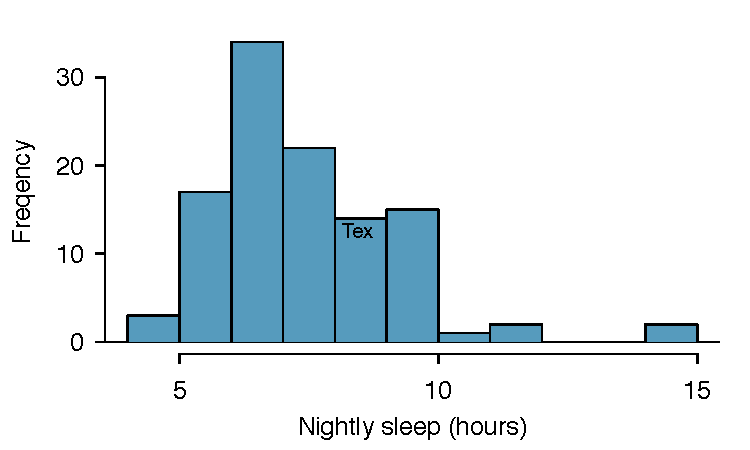
\includegraphics[width=0.7\textwidth]{ch_inference_foundations_oi_biostat/figures/histOfSleepForCollegeThatWasCheckingForMoreThan7Hours/histOfSleepForCollegeThatWasCheckingForMoreThan7Hours}
\caption{Distribution of a night of sleep for 110 college students. These data are strongly skewed.\index{skew!example: strong}}
\label{histOfSleepForCollegeThatWasCheckingForMoreThan7Hours}
\end{figure}

The normal model for the sample mean can be used here because: (1) this is a simple random sample from less than 10\% of the student body, the observations are independent; (2)~the sample size in the sleep study is sufficiently large since it is greater than 30; (3)~The data show strong skew in Figure~\ref{histOfSleepForCollegeThatWasCheckingForMoreThan7Hours} and the presence of a couple of outliers. This skew and the outliers are acceptable for a sample size of $n=110$. 

\begin{exercise} \label{findSEOfFirstSleepStudyCheckingGreaterThan7Hours}
In the sleep study, the sample standard deviation was 1.75 hours and the sample size is 110. Calculate the standard error of $\bar{x}$.\footnote{The standard error can be estimated from the sample standard deviation and the sample size: $SE_{\bar{x}} = \frac{s_x}{\sqrt{n}} = \frac{1.75}{\sqrt{110}} = 0.17$.}
\end{exercise}

The hypothesis test for the sleep study will be evaluated using a significance level of $\alpha = 0.05$. If $H_0$ is true, the sample mean is from a distribution that is nearly normal with mean 7 and standard deviation of about $SE_{\bar{x}} = 0.17$. Such a distribution is shown in Figure~\ref{pValueOneSidedSleepStudy}.

\begin{figure}[hht]
   \centering
   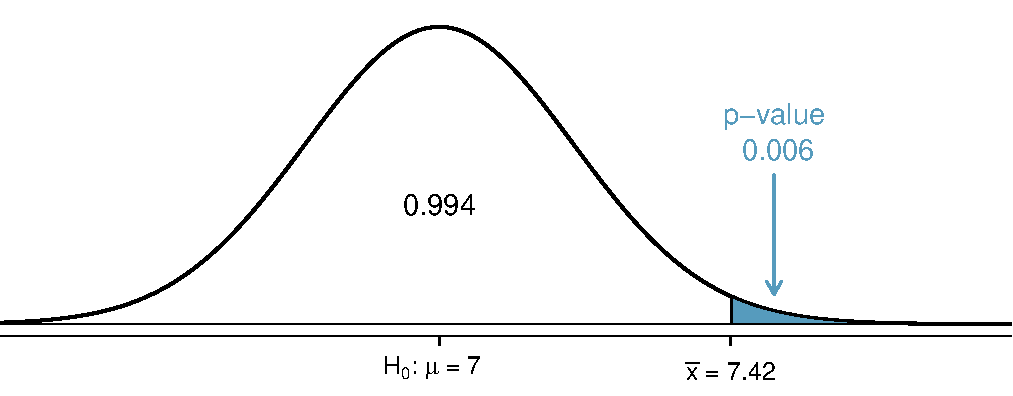
\includegraphics[width=0.83\textwidth]{ch_inference_foundations_oi_biostat/figures/pValueOneSidedSleepStudy/pValueOneSidedSleepStudy}
   \caption{If the null hypothesis is true, then the sample mean $\bar{x}$ came from this nearly normal distribution. The right tail describes the probability of observing such a large sample mean if the null hypothesis is true.}
   \label{pValueOneSidedSleepStudy}
\end{figure}

The shaded tail in Figure~\ref{pValueOneSidedSleepStudy} represents the chance of observing such a large mean if the null hypothesis is true. That is, the shaded tail represents the \mbox{p-value}. All means larger than the sample mean, $\bar{x} = 7.42$ are shaded, because they are more favorable to the alternative hypothesis than the observed mean.

The $p$-value is the tail area of this normal distribution, calculated using techniques in Section~\ref{normalDist}. First compute the Z-score of the sample mean, $\bar{x} = 7.42$:
\begin{eqnarray*}
Z = \frac{\bar{x} - \text{null value}}{SE_{\bar{x}}} = \frac{7.42 - 7}{0.17} = 2.47
\end{eqnarray*}
Using the normal probability table, the lower unshaded area is  be 0.993. Thus the shaded area is $1-0.993 = 0.007$. {\em If the null hypothesis is true, the probability of observing a sample mean at least as large as 7.42 hours for a sample of 110 students is only 0.007.}\index{p-value!interpretation example} That is, if the null hypothesis is true, we would not often see such a large mean.

The hypotheses are tested by comparing the $p$-value to the significance level. Because the $p$-value is less than the significance level ($p$-value $=0.007 < 0.05=\alpha$), the null hypothesis is rejected. The data are so unusual with respect to the null hypothesis that they casts serious doubt on $H_0$ and provide strong evidence favoring $H_A$.

\begin{termBox}{\tBoxTitle{$p$-value as a tool in hypothesis testing}
The smaller the p-value, the stronger the data favor $H_A$ over $H_0$. A small p-value (usually $<0.05$) corresponds to sufficient evidence to reject $H_0$ in favor of $H_A$.}
\index{hypothesis testing!p-value|)}
\end{termBox}

\begin{tipBox}{\tipBoxTitle{It is useful to first draw a picture to find the p-value}
It is useful to draw a picture of the distribution of $\bar{x}$ as though $H_0$ was true (i.e.~$\mu$~equals the null value), and shade the region (or regions) of sample means that are at least as favorable to the alternative hypothesis. These shaded regions represent the p-value.}
\end{tipBox}


The $p$-value is constructed in such a way that it can be directly compared to the significance level ($\alpha$) to determine whether or not to reject $H_0$. This method ensures that the Type~1 Error rate does not exceed the significance level standard. 

\begin{figure}[ht]
   \centering
   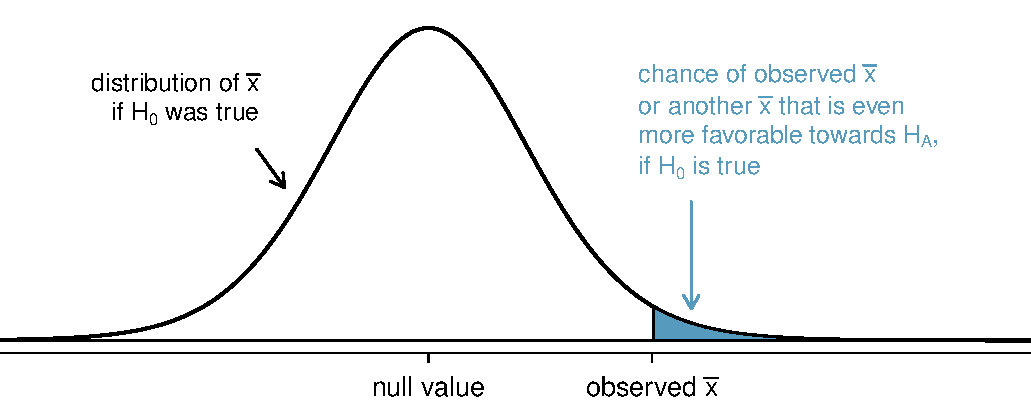
\includegraphics[width=0.9\textwidth]
{ch_inference_foundations_oi_biostat/figures/pValueOneSidedSleepStudyExplained/pValueOneSidedSleepStudyExplained}
   \caption{To identify the p-value, the distribution of the sample mean is considered as if the null hypothesis was true. Then the p-value is defined and computed as the probability of the observed $\bar{x}$ or an $\bar{x}$ even more favorable to $H_A$ under this distribution.}
   \label{pValueOneSidedSleepStudyExplained}
\end{figure}

\begin{exercise}
If the null hypothesis is true, how often should the p-value be less than 0.05?\footnote{About 5\% of the time. If the null hypothesis is true, then the data only has a 5\% chance of being in the 5\% of data most favorable to $H_A$.}
\index{data!school sleep|)}
\end{exercise}

\begin{exercise}
Suppose we had used a significance level of 0.01 in the sleep study. Would the evidence have been strong enough to reject the null hypothesis? (The p-value was 0.007.) What if the significance level was $\alpha = 0.001$? \footnote{We reject the null hypothesis whenever $p$-$value < \alpha$. Thus, we would still reject the null hypothesis if $\alpha = 0.01$ but not if the significance level had been $\alpha = 0.001$.}
\end{exercise}

Here is an example with a two-sided alternative. In one-sided tests, the single tail in the direction of the alternative hypothesis is shaded. For example, when the alternative had the form $\mu > 7$, then the p-value was represented by the upper tail (Figure~\ref{pValueOneSidedSleepStudyExplained}).  In a two-sided test, since evidence in either direction is favorable to $H_A$ so both tails are shaded.

\begin{exercise} \label{2ndSchSleepHypSetupExercise}
The earlier example investigated whether the students at a school slept longer than 7 hours each night. Suppose a second group of researchers wanted to evaluate whether the students at their college differ from the norm of 7 hours. Write the null and alternative hypotheses for this investigation.\footnote{Because the researchers are interested in any difference, they should use a two-sided setup: $H_0: \mu = 7$, $H_A: \mu \neq 7$.}
\end{exercise}

\begin{example}{Suppose the second college randomly sampled 122 students and found a mean of $\bar{x} = 6.83$ hours and a standard deviation of $s=1.8$ hours. Does this provide strong evidence against $H_0$ in Guided Practice~\ref{2ndSchSleepHypSetupExercise}? Use a significance level of $\alpha=0.05$.}
The required assumptions hold here. (1) A simple random sample of less than 10\% of the student body means the observations are independent. (2) The sample size is 122, which is greater than 30. (3) Based on the information in the earlier distribution, the sample size will be sufficient to to mitigate the effect of skewness or outliers.

The standard error of the estimate is $SE_{\bar{x}} = \frac{s}{\sqrt{n}} = 0.16$;  a picture  representing the $p$-value is shown in Figure~\ref{2ndSchSleepHTExample}. Both tails are shaded. An estimate of 7.17 or more provides at least as strong of evidence against the null hypothesis and in favor of the alternative as the observed estimate, $\bar{x} = 6.83$.

The calculation the tail areas starts by first finding the lower tail corresponding to $\bar{x}$:
\begin{eqnarray*}
Z = \frac{6.83 - 7.00}{0.16} = -1.06 \quad\stackrel{table}{\rightarrow}\quad \text{left tail} = 0.1446
\end{eqnarray*}
Because the normal model is symmetric, the right tail will have the same area as the left tail. The $p$-value is found as the sum of the two shaded tails:
\begin{eqnarray*}
\text{p-value} = \text{left tail} + \text{right tail} = 2\times(\text{left tail}) = 0.2892
\end{eqnarray*}
This p-value is relatively large (larger than $\alpha=0.05$), so  $H_0$ is not rejected. That is, if $H_0$ is true, it would not be very unusual to see a sample mean this far from 7 hours simply due to sampling variation. 

\index{data!school sleep|)}

\begin{figure}
   \centering
   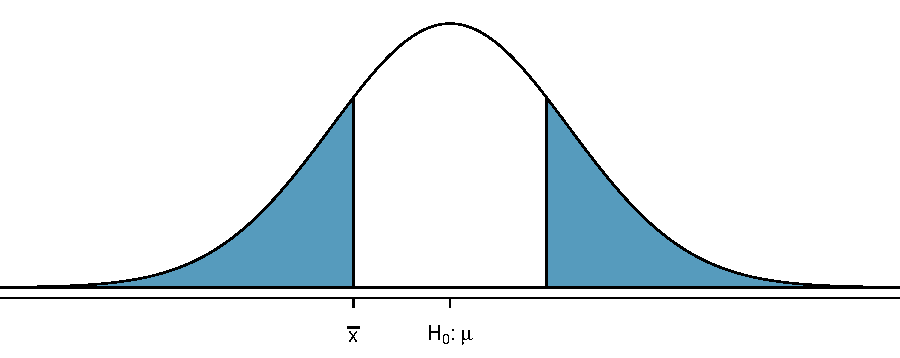
\includegraphics[width=0.9\textwidth]
   {ch_inference_foundations_oi_biostat/figures/2ndSchSleepHTExample/2ndSchSleepHTExample}
   \caption{$H_A$ is two-sided, so \emph{both} tails must be counted for the p-value.}
   \label{2ndSchSleepHTExample}
\end{figure}

\end{example}

\begin{example}{It not correct to change two-sided tests to one-sided tests after observing the data.  This example explores the consequences of making that error. Using $\alpha=0.05$, freely switching from two-sided tests to one-sided tests cause twice as many Type~1 Errors as intended.} \label{swappingHypAfterDataDoublesType1ErrorRate}
Suppose the sample mean was larger than the null value, $\mu_0$ (e.g. $\mu_0$ would represent~7 if $H_0$:~$\mu = 7$). Flipping to a one-sided test $H_A$: $\mu > \mu_0$, any observation with a Z-score greater than 1.65, would lead to  rejecting  $H_0$. If the null hypothesis is true, the null hypothesis is incorrectly rejected about 5\% of the time when the sample mean is above the null value, as shown in Figure~\ref{type1ErrorDoublingExampleFigure}.

Suppose the sample mean was smaller than the null value.  Changing to a one-sided alternative $H_A$: $\mu < \mu_0$, a $\bar{x}$ with a Z-score smaller than -1.65, we would lead to rejecting $H_0$. If the null hypothesis is true, this would happen about 5\% of the time.

These two scenarios, it can be shown that a Type~1 Error will occur about $5\%+5\%=10\%$ of the time whenever the test is swapped for ``best'' one-sided test for the data. This is twice the error rate prescribed with significance level: $\alpha=0.05$.

\begin{figure}
   \centering
   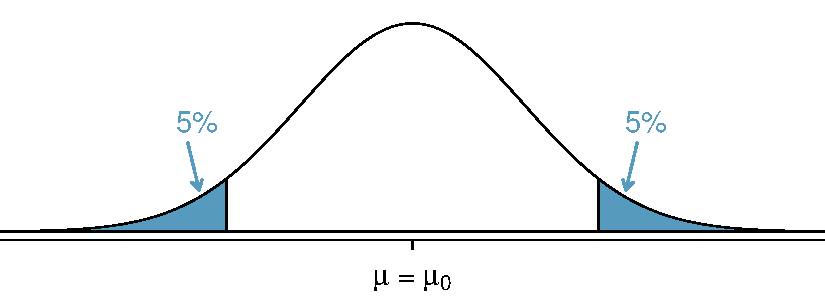
\includegraphics[width=0.7\textwidth]{ch_inference_foundations_oi_biostat/figures/type1ErrorDoublingExampleFigure/type1ErrorDoublingExampleFigure}
   \caption{The shaded regions represent areas where we would reject $H_0$ under the bad practices considered in Example~\ref{swappingHypAfterDataDoublesType1ErrorRate} when $\alpha = 0.05$.}
   \label{type1ErrorDoublingExampleFigure}
\end{figure}

\end{example}

\begin{caution}{One-sided hypotheses are allowed only \emph{before} seeing data}
{After observing data, it is tempting to turn a two-sided test into a one-sided test. Avoid this temptation. Hypotheses must be set up \emph{before} observing the data. If~they are not, the test should be two-sided.}
\end{caution}


\subsection{Hypothesis testing using confidence intervals}

When a 95\% confidence interval is used  for testing in the situation where $H_0$ is true, an error is made whenever the point estimate is at least 1.96 standard errors away from the population parameter. This happens about 5\% of the time (2.5\% in each tail). Similarly, using a 99\% confidence interval to evaluate a hypothesis is equivalent to a significance level of $\alpha = 0.01$.

A confidence interval provides important but limited information about a test.  Consider the following two scenarios:
\begin{itemize}
\setlength{\itemsep}{0mm}
\item The null value (the parameter value under the null hypothesis) is in the 95\% confidence interval but just barely, so $H_0$ is not rejected. It would be useful to report in some way,however, that it was a close decision.
\item The null value is very far outside of the interval, so we reject $H_0$. This dise not communicate that the decision was not even close. Such a case is depicted in Figure~\ref{whyWeWantPValue}.
\end{itemize}
The $p$-value introduced in Section~\ref{formalHypothesisTesting}, is helpful in these cases. The $p$-value method also extends to hypothesis tests where confidence intervals cannot be easily constructed or applied.

\begin{figure}[hht]
\centering
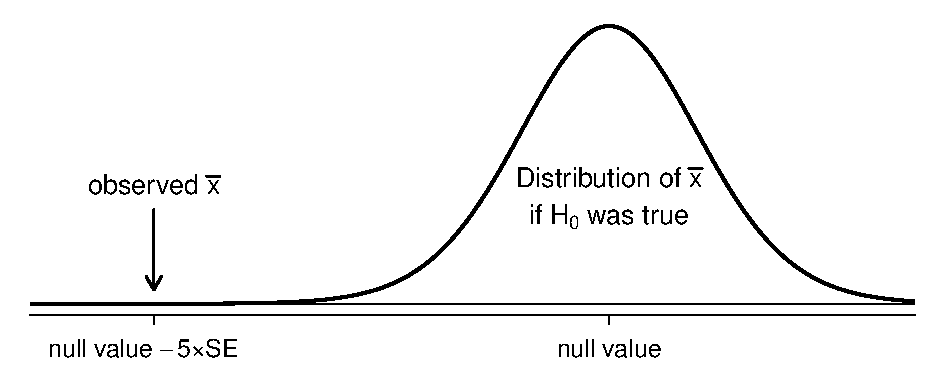
\includegraphics[width=0.75\textwidth]
{ch_inference_foundations_oi_biostat/figures/whyWeWantPValue/whyWeWantPValue}
\caption{It would be helpful to quantify the strength of the evidence against the null hypothesis. In this case, the evidence is extremely strong.}
\label{whyWeWantPValue}
\end{figure}


%% the next section is taken directly from OI and needs to be revised, and trimmed.

\subsection{Choosing a significance level}
\label{significanceLevel}

\index{hypothesis testing!significance level|(}
\index{significance level|(}

Choosing a significance level for a test is important in many contexts, and the traditional level is 0.05. However, it is often helpful to adjust the significance level based on the application. We may select a level that is smaller or larger than 0.05 depending on the consequences of any conclusions reached from the test.

If making a Type~1 Error is dangerous or especially costly, we should choose a small significance level (e.g. 0.01). Under this scenario we want to be very cautious about rejecting the null hypothesis, so we demand very strong evidence favoring $H_A$ before we would reject $H_0$.

If a Type~2 Error is relatively more dangerous or much more costly than a Type~1 Error, then we should choose a higher significance level (e.g. 0.10). Here we want to be cautious about failing to reject $H_0$ when the null is actually false.

In the early testing of the effectiveness of a relatively benign drug in treating a disease, it may be important to continue further testing even if the evidence for a beneficial effect is not quite as strong as is used in more traditional significance.  If scientists studying the drug know that initial positive results will have to be confirmed in larger study, they might use $\alpha = 0.10$ instead of the stricter $0.05$.  If, on the other hand, the drug is likely to show serious, perhaps even fatal side effects, it may be prudent to use $\alpha = 0.01$ in initial testing, to reduce the chance of concluding that the drug works when it is not effective.


\begin{tipBox}{\tipBoxTitle[]{Significance levels should reflect consequences of errors}
The significance level selected for a test should reflect the consequences associated with Type~1 and Type~2 Errors.}
\end{tipBox}


\index{significance level|)}
\index{hypothesis testing!significance level|)}
\index{hypothesis testing|)}



\end{spacing}
 


